\documentclass[12pt]{article}
\usepackage{../../../lecture_notes}
\usepackage{../../../math}
\usepackage{../../../uark_colors}
\hypersetup{
  colorlinks = true,
  allcolors = ozark_mountains,
  breaklinks = true,
  bookmarksopen = true
}
\newcommand{\answer}[1]{{\color{blue_winged_teal}\textbf{Answer:} #1}}
\newcommand{\pts}[1]{{\color{zinc500}#1}}

\begin{document}
\begin{center}
  {\Huge\bf Midterm - Fall 2024}
  
  \smallskip
  {\large\it  ECON 5783 — University of Arkansas}
\end{center}

\medskip
\begin{enumerate}
%   \item Say a researcher wants to model the conditional expectation of wages given gender, college degree, and age. What should the author do if they want to `flexibly' model the conditional expectation function? 

  \item A researcher wants to test the folk-wisdom that playing classical music for children benefits their future academic achievement. The researcher surveys parents and records their high-school GPA ($Y_i$) and whether or not they listened to classical music ($D_i$) as a child.
  \begin{enumerate}
    \item In this context, describe in words what the potential outcomes, $Y_i(0)$ and $Y_i(1)$, are.
    
    \answer{
      $Y_i(0)$ is the child's high school GPA if the family \emph{did not} play classical music. $Y_i(1)$ is the child's high school GPA if the family \emph{did} played classical music. 
    }
    
    \item Do you think the difference-in-means estimator would be biased in this context? If so, which direction do you the treatment effect estimate is biased?
    
    \answer{
      I think the difference-in-means estimator would be biased in this context. I think that parents that play classical music would tend to have high income than those that do not. Therefore, the average $Y_i(0)$ would likely be higher for the treated children, so selection bias would be positive. 
    }
    
    \item Why might a table of summary statistics consisting of sample means of observables, broken down by $D_i = 0$ and $D_i = 1$, be useful in this setting?
    
    \answer{
      A table of summary statistics could be useful in this setting to allow the reader to see if the families that play classical music \emph{actually} look different than those that do not. The table will be more informative the more rich the summary statistics are.
    }
  \end{enumerate}

  \medskip
  \item Say you believe the conditional independence assumption $(Y_i(1), Y_i(0)) \Perp D_i \ \vert \ X_i$ holds. 
  \begin{enumerate}
    \item In words, describe what the steps you would take to use a nearest-neighbor matching-based estimator of the treatment effect
    
    \answer{
      First, I would select a set of important control variables $X_i$. For each treated unit, I would find the control unit that is closest to that unit in terms of covariates. This could be done by comparing units by their Mahalanobis distance between the covariates. 

      Doing this for all treated units would create a matched control set. Then I would do a difference-in-means estimate between the treated and the matched-control set.
    }
    
    \item Say a reader had some concern that overlap would hold in the given application. Why might a balance table be useful for this reader? 
    
    \answer{
      Since we are doing nearest-neighbor matching, we might be concerned that the quality of matches is poor. A balance table will show the reader how close the treated and matched-control group arew in terms of their covariate values.
    }
  \end{enumerate}
  
  \medskip
  \item The simplest treatment effect estimator in a setting where you believe the conditional independence assumption is to difference-in-means estimation for individuals with the same values of $X_i = x$ (e.g. separate estiamtes for male and females). The overall treatment effect is formed as a weighted average of the estimates $\widehat{\text{CATE}}(x)$.
  \begin{enumerate}
    \item Describe why the curse of dimensionality makes this infeasible in many settings.
    
    \answer{
      As the dimension of the covariate vector $X_i$ gets larger, the number of units with $X_i = x$ will get smaller and smaller. In many cases, there will fail to be control units with the same value of $x$. This makes this strategy infeasible for $X_i$ of large-dimension. Instead, we must rely on an alternative estimator; e.g. propensity-score matching, inverse probaiblity of treatment-weighting, or regression adjustment.
    }
  \end{enumerate}
\end{enumerate}


\bigskip
\noindent
For the following questions refer to Figure \ref{fig:huh_reif_2021}. 
These are two figures from the paper ``Teenage Driving, Mortality, and Risky Behaviors'' in AER: Insights. 
The authors want to study teenage driving on risky behavior and mortality. 
They use a state's minimum driving-age as the cutoff and age as a running variable. 
Those under the minimum age law can not drive and those above can. 

\medskip
\begin{enumerate}
  \setcounter{enumi}{3}
  \item Figure \ref{fig:huh_reif_2021}(a) presents their main results (separately for male and female drivers). 
  They argue that the jump in deaths by motor vehicle accidents is from the driver's ability to drive. 
  What assumptions do we need to make for this RD to identify the causal effect? 
  I am not looking for the `generic' assumption here; I want you to describe the assumption in the context of the research question.

  \answer{
    For this treatment effect estimator we need the continuity assumption.  That is, we need the average death rate in both the world without the ability to drive and with the ability to drive to evolve smoothly as a function of age around the MDA cutoff.
  }
 
  \medskip
  \item The authors present figure \ref{fig:huh_reif_2021}(b) that shows the jump in deaths from `Any Cause' is the same magnitude as the jump \emph{just} from motor vehicle accidents. 
  Do you think this figure helps strengthen their causal claim? Why or why not? 

  \answer{
    I think this figure helps strengthen their causal claim. We might be concerned that other behaviors might change at the same time as the MDA. 
    By showing that the jump at the cut-off is due primarily to driving deaths and not other kinds of deaths, the authors have ruled out many other potential confounding factors.
  }
\end{enumerate}

\medskip
\begin{figure}[htb!]
  \caption{Results from Huh and Reif (2021, AER Insights)}
  \label{fig:huh_reif_2021}
  \begin{center}
    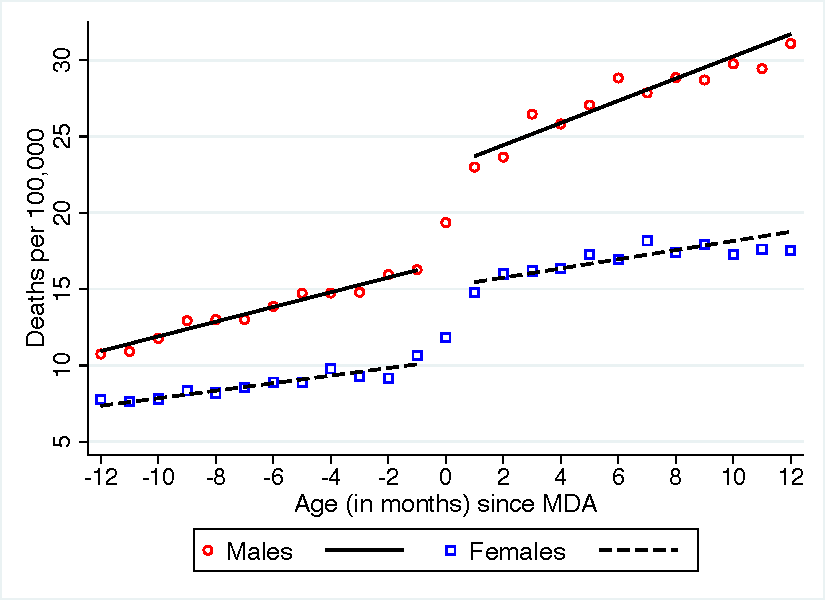
\includegraphics[width = 0.6\textwidth]{rd_mva_male_female.pdf}
    \subcaption{Deaths by Motor Vehicle Accidents}
  \end{center}

  \begin{center}
    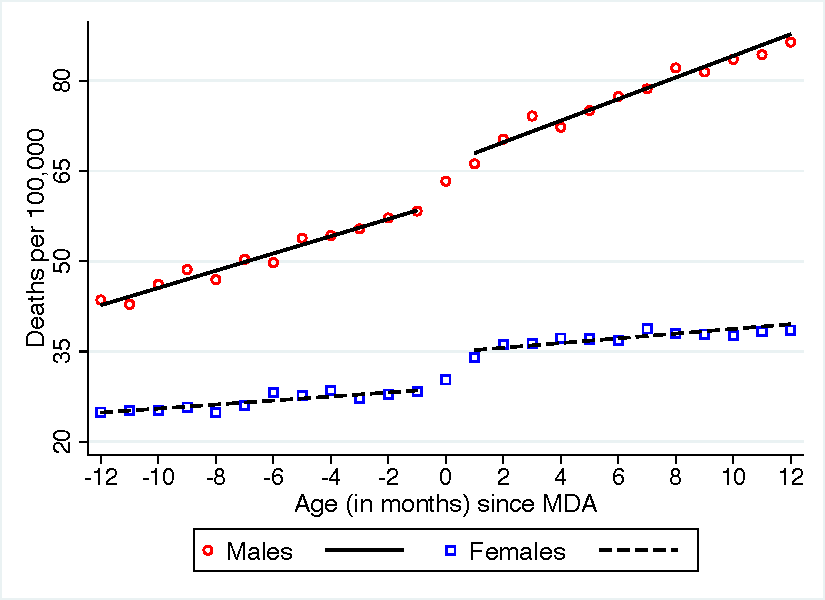
\includegraphics[width = 0.6\textwidth]{rd_any_male_female.pdf}
    \subcaption{Deaths by Any Cause}
  \end{center}
\end{figure}

\end{document}
